\documentclass[tikz]{standalone}

\usepackage{amsmath}
\usepackage{circuitikz}
\usepackage{siunitx}

\let\Re\undefined
\DeclareMathOperator{\Re}{\operatorname{Re}}

\begin{document}
	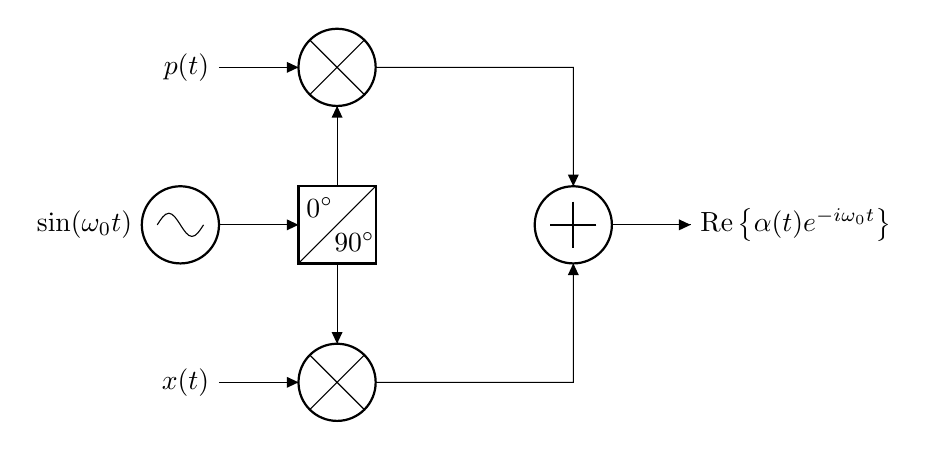
\begin{tikzpicture}
		\draw (2.5,0) node[left]{$x(t)$} (4,0)
            node[mixer](mixer){};
        \draw (2.5,0) to[short] (mixer.west) node[inputarrow, anchor=tip]{};
        \draw (2.5,2) node[oscillator, label={left:$\sin(\omega_0t)$}](osc){} to[short] (mixer.west |- osc) node[inputarrow]{} node[twoportsplitshape, anchor=west, circuitikz/t1=$\SI{0}{\degree}$, circuitikz/t2=$\SI{90}{\degree}$](splitter){};
        \draw (splitter.south) to[short] (mixer.north) node[inputarrow, rotate=-90]{};
        \draw (2.5,4) node[left]{$p(t)$} to[short] (0,4-|mixer.west) node[inputarrow]{} node[mixer, anchor=west](mixer2){};
        \draw (splitter.north) to[short] (mixer2.south) node[inputarrow, rotate=90]{};
        \draw (splitter) ++(3,0) node[adder](adder){};
        \draw (mixer.east) to[short] (mixer-|adder) to[short] (adder.south) node[inputarrow, rotate=90]{};
        \draw (mixer2.east) to[short] (mixer2-|adder) to[short] (adder.north) node[inputarrow, rotate=-90]{};
        \draw (adder.east) to[short] ++(1,0) node[inputarrow]{} node[right]{$\operatorname{Re}\left\{\alpha(t)e^{-i\omega_0t}\right\}$};
	\end{tikzpicture}
\end{document}
